% Revisiting Gene Set Enrichment Analysis
% Section 4 of the committee meeting, 2026-07-30.
%
% Ground rules: Beamer, SIMPLE construction (content over polish), bibliography
% included. Every \includegraphics points at figures/<name>.pdf, all built with
% provenance via `snakemake -s figures.smk all`. Build the deck with:
%     snakemake -s figures.smk all -c4 && latexmk -pdf deck.tex
%
% Naming: cox / cox-reverse (= Plackett-Luce partial likelihood).
% Cartoons in the review-surface artifact are mockups; these figures are stubs
% until the T1-T5 / migration tasks fill them in.

\documentclass[aspectratio=169]{beamer}
\usetheme{default}
\usecolortheme{seahorse}
\setbeamertemplate{navigation symbols}{}
\setbeamertemplate{caption}{\raggedright\insertcaption\par}

% Slide numbers (current/total) in the bottom-right of every frame.
\setbeamertemplate{footline}{%
  \hfill\usebeamercolor[fg]{page number in head/foot}%
  \insertframenumber/\inserttotalframenumber\kern1em\vskip2pt}

\usepackage{graphicx}
\usepackage{booktabs}
\usepackage{amsmath}
\graphicspath{{figures/}{resources/}}

% Fixed-footprint figure: every figure is centred in the SAME box
% (0.70\textwidth x 0.72\textheight) with keepaspectratio, so figures line up and
% captions always start at the same height regardless of a figure's aspect ratio.
% See scripts/check_figures.py, which enforces the aspect band this box assumes.
\newcommand{\slidefig}[1]{%
  \par\centering
  \parbox[c][0.72\textheight][c]{\textwidth}{%
    \centering\includegraphics[width=0.70\textwidth,height=0.72\textheight,keepaspectratio]{#1}}%
  \par}

\title{Revisiting Gene Set Enrichment Analysis}
\subtitle{How much resolution do we need? scores $\to$ ranks $\to$ binary}
\author{Karl Tayeb}
\date{Committee meeting -- 30 July 2026}

\begin{document}

\begin{frame}[plain]
  \titlepage
\end{frame}

% =====================================================================
\section{Setup \& motivation}
% =====================================================================

\begin{frame}{GSEA: what it's for}
  \begin{itemize}
    \item Introduce via the $2\times 2$ contingency table (DE vs.\ in-set).
    \item Two goals:
      \begin{itemize}
        \item \textbf{Interpretation} -- summarize a gene list into a pathway.
        \item \textbf{Aggregation} -- detect small coordinated changes.
      \end{itemize}
  \end{itemize}
\end{frame}

\begin{frame}{Covid Example}
  \only<1-3>{%
    \centering
    \begin{minipage}[t]{0.56\textwidth}\centering
      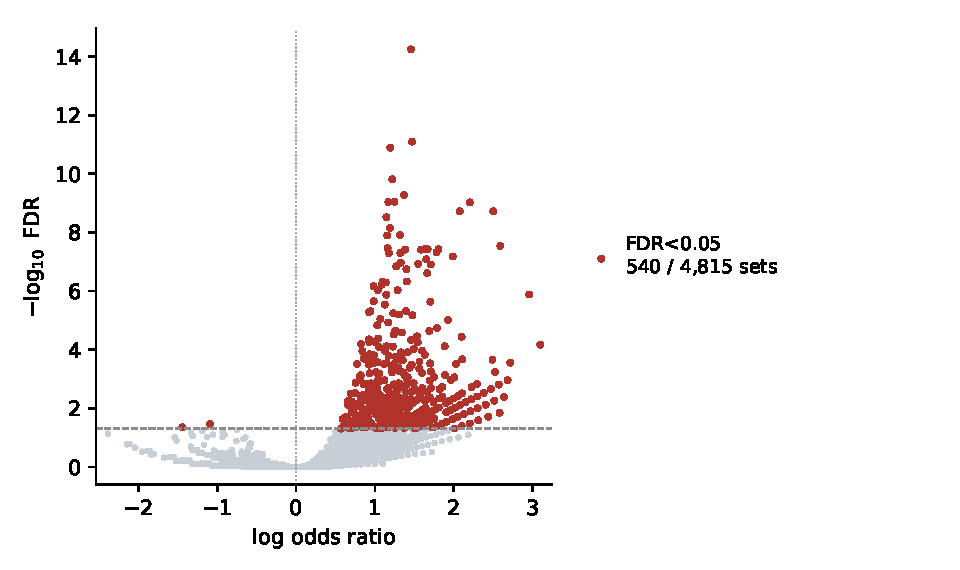
\includegraphics[height=0.56\textheight,width=\linewidth,keepaspectratio]{covid_volcano}%
      \\[-0.1em]{\scriptsize\color{black!60} marginal ORA: \textbf{540/4{,}815} sets sig.\ (11\%)}
    \end{minipage}\hfill
    \begin{minipage}[t]{0.40\textwidth}\centering
      \only<1>{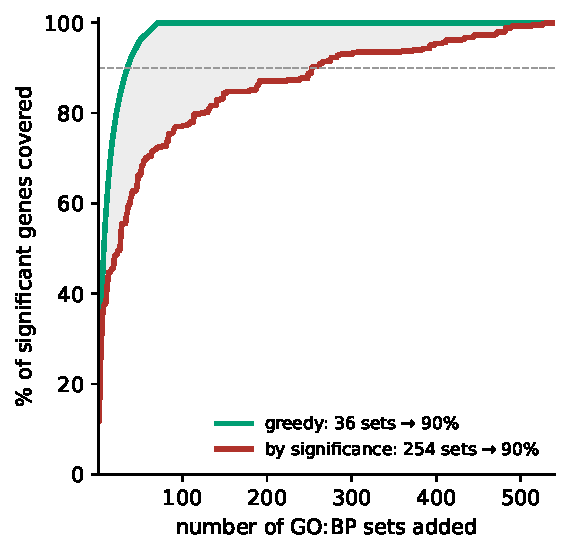
\includegraphics[height=0.56\textheight,width=\linewidth,keepaspectratio]{covid_redundancy}}%
      \only<2>{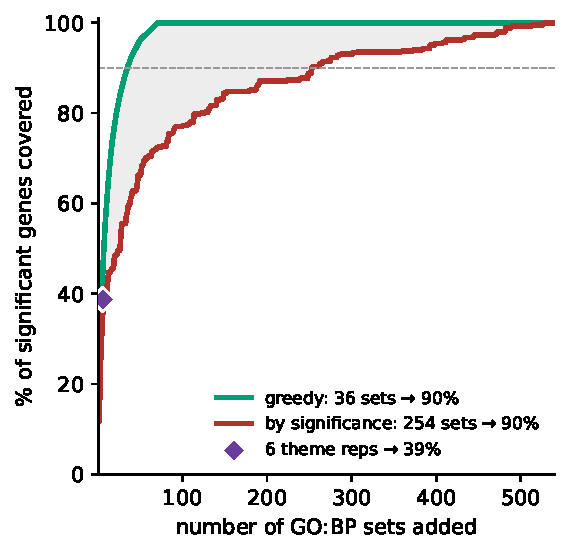
\includegraphics[height=0.56\textheight,width=\linewidth,keepaspectratio]{covid_redundancy1}}%
      \only<3>{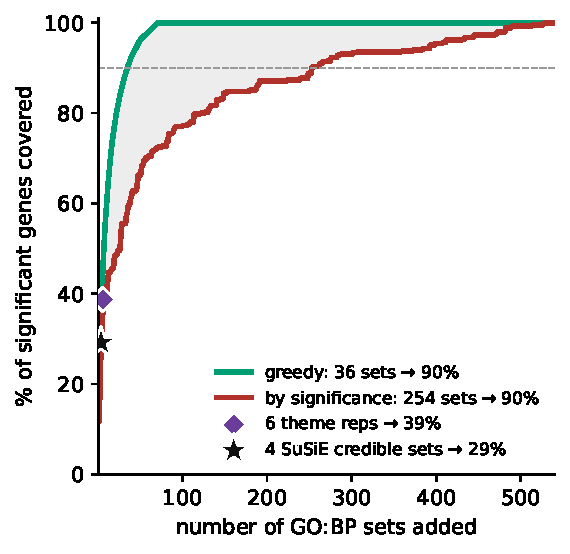
\includegraphics[height=0.56\textheight,width=\linewidth,keepaspectratio]{covid_redundancy2}}%
      \\[-0.1em]{\scriptsize\color{black!60}
        \only<1>{\textbf{254} sig.-ordered sets to cover 90\%}%
        \only<2>{\textbf{6} theme reps $\to$ 39\%}%
        \only<3>{\textbf{4} SuSiE credible sets $\to$ 29\%}}
    \end{minipage}%
  }%
  \only<4>{\slidefig{fig_ora_redundancy_marginal}}%
  \only<5>{\slidefig{fig_ora_redundancy_causal}}%
  \par\medskip
  {\footnotesize
  \only<1>{\textbf{Real SARS-CoV-2 GO:BP ORA.} Marginal enrichment flags \textbf{540 of
  4{,}815} sets (\textbf{11\%}) -- a huge cloud (\emph{left}). Coverage curve
  (\emph{right}): by significance you add \textbf{254} sets to cover 90\% of the
  significant genes. Redundant -- and inflated by \emph{non-independence} (overlapping
  sets are correlated tests).}%
  \only<2>{\textbf{The hits are a few themes.} Clustering the top sets, \textbf{6}
  theme representatives already cover \textbf{39\%} of the significant genes (purple) --
  the signal is low-dimensional.}%
  \only<3>{\textbf{A joint model is compact.} \textbf{4} SuSiE credible sets cover
  \textbf{29\%} (star): a handful of components replaces the hundreds of redundant
  marginal hits.}%
  \only<4>{\textbf{Simulate the same picture.} Two-group model over \textbf{4{,}870}
  GO:BP sets; marginal ORA flags \textbf{556} (\textbf{11\%}) -- the same
  uninterpretable cloud, but now we know the ground truth.}%
  \only<5>{\textbf{The truth: 10 causal sets} (2 large / 3 medium / 5 small). The 556
  marginal hits are redundant re-coverings of these few signals -- the motivation for a
  joint SuSiE model (next).}%
  }
\end{frame}

\begin{frame}{SuSiE handles redundancy}
  \slidefig{tcellenrich}
  \par\medskip
  {\footnotesize One \textbf{joint} sparse regression (SuSiE prior) replaces
  thousands of marginal tests: each credible set (L1--L4) captures an
  \emph{independent} signal and may hold several competing/redundant sets.
  Redundant within, complementary across -- simpler, more precise biology.
  Ties back to Logistic SuSiE (\S1) and GLM SuSiE / GIBSS (\S3).}
\end{frame}

\begin{frame}{Two jobs for enrichment -- and where the 2$\times$2 fails}
  \slidefig{fig_two_regimes}
  \par\medskip
  {\footnotesize A few large effects (A) cross any threshold -- the 2$\times$2 sees
  them. A small coordinated shift (B) crosses nothing -- the 2$\times$2 is blind,
  even though the set is really shifted. Thresholding discards exactly the
  aggregation signal: the motivation for richer resolutions.}
\end{frame}

\begin{frame}{Data arrives at different resolutions}
  \begin{itemize}
    \item scores $\to$ rankings $\to$ hit-lists.
    \item Down the ladder: less \textbf{information}, more \textbf{robustness}
      / fewer assumptions.
    \item This tradeoff is the spine of the talk; it decides whether we can do
      the \textbf{second} job (aggregation), not just the first.
  \end{itemize}
\end{frame}

\begin{frame}{Covariate-moderated two-group model (working model)}
  \[
    \hat b_i \mid b_i \sim N(b_i, s_i^2), \quad
    b_i \sim (1-z_i)\,\delta_0 + z_i\, f_1, \quad
    z_i \sim \mathrm{Bernoulli}(\theta^\top x_i), \quad
    \theta \sim \mathrm{SuSiE}.
  \]
  \begin{itemize}
    \item This is \textbf{Aim 2b} (R01): joint GSEA directly from effect sizes
      $(\hat b_i, s_i)$ -- avoid the thresholding that discards information and
      needs a chosen cutoff (Aim 2a = logistic SuSiE on a hit-list).
    \item Caveat, stated up front: gene scores are \emph{probably not
      independent}.
    \item Signal driven by $N(\mu, 0.1)$ (location) or $N(0,\sigma^2)$ (scale).
  \end{itemize}
\end{frame}

% =====================================================================
\section{The resolution spectrum}
% =====================================================================

\begin{frame}{One dataset, three resolutions}
  \slidefig{fig06_resolution_spectrum}
  \par\medskip
  {\footnotesize Same genes as scores $\to$ ranks $\to$ binary; logistic
  $\leftrightarrow$ interval censoring.}
\end{frame}

\begin{frame}{Modeling scores directly}
  \begin{itemize}
    \item Two-group is the ``correct'' model: spike $\delta_0$ + slab $f_1$.
    \item But you must \textbf{estimate $f_1$} -- the hardest case in the talk.
  \end{itemize}
\end{frame}

\begin{frame}{Misspecifying $f_1$ is the real risk (not identifiability)}
  \slidefig{fig08_misspecification}
  \par\medskip
  {\footnotesize With a parametric $f_1$ the model is identifiable; the practical
  danger is the wrong family. A location-family fit to scale-driven data collapses
  ($\sim$0.04 PIP), while cox-reversed - which models no $f_1$ - stays robust.}
\end{frame}

\begin{frame}{What logistic actually estimates}
  \slidefig{fig09_logistic_estimand}
  \par\medskip
  {\footnotesize Log-odds of \emph{exceeding} $\tau$, not of being DE.
  Overlapping $f_0/f_1$ give false positives / negatives.}
\end{frame}

\begin{frame}{The cost of discretizing -- localization (causal PIP)}
  \slidefig{fig10_pip_vs_threshold}
  \par\medskip
  {\footnotesize Four difficulty-matched cells (gene set size $\times$ loc/scale)
  on \textbf{c2}, 200 sims each. Two-group (continuous $z$) is the ceiling;
  discretizing costs power on \emph{loc} but is nearly free on \emph{scale};
  cox-full (no threshold) is weak -- the threshold is what powers the forward cox.}
\end{frame}

\begin{frame}{The cost of discretizing -- detection (logBF ROC)}
  \slidefig{fig11_cod_roc}
  \par\medskip
  {\footnotesize Same cells: can the SER log-BF separate enrichment from null?
  (legend $=$ AUC). Same ordering as the PIP view -- two-group best, discretizing
  cheap on scale / costly on loc, linear-on-$z$ near chance on scale, cox-full
  near chance.}
\end{frame}

% =====================================================================
\section{Rankings}
% =====================================================================

\begin{frame}{Binary is interval-censored}
  \begin{itemize}
    \item $Y=1$: arrival in $[0,T]$. \quad $Y=0$: censored at $T$.
    \item Partial rankings keep the ordering the hit-list discards.
    \item Introduces the \textbf{cox} rank model (= Plackett--Luce partial
      likelihood).
  \end{itemize}
\end{frame}

\begin{frame}{cox vs.\ logistic}
  \begin{itemize}
    \item At stringent $\tau$, $P(Y_i=1)\approx z_i$ -- the two coincide.
    \item cox's edge: \textbf{robustness to a permissive threshold}.
  \end{itemize}
\end{frame}

\begin{frame}{cox or cox-reverse?}
  \begin{itemize}
    \item \textbf{cox}: most $\to$ least significant.
    \item \textbf{cox-reverse}: least $\to$ most significant (most significant
      genes become most influential).
    \item Next three slides: why cox-reverse is the safer default.
  \end{itemize}
\end{frame}

\begin{frame}{The PH assumption breaks (location vs.\ scale)}
  \slidefig{fig14_hazard_loc_scale}
  \par\medskip
  {\footnotesize Forward blows up for the most informative genes; reverse
  stays stable -- shown for location- and scale-driven signal.}
\end{frame}

\begin{frame}{Late arrivals dominate the score}
  \slidefig{fig15_late_arrival}
  \par\medskip
  {\footnotesize Last arrival $\sim O(\log n)$ vs.\ first $\sim O(1)$.
  A late arrival = many unlikely picks in a row. (derivations: B1, B2)}
\end{frame}

\begin{frame}{Reverse-rank, and censor the tail}
  \begin{itemize}
    \item Right-censoring suits cox, where high-leverage observations are null.
    \item Reverse ranking is desirable because
      \begin{itemize}
        \item[(1)] it is a \textbf{milder PH violation}, and
        \item[(2)] it makes the \textbf{most significant genes most
          influential}.
      \end{itemize}
  \end{itemize}
\end{frame}

% =====================================================================
\section{Results \& payoff}
% =====================================================================

\begin{frame}{When PH holds, it's calibrated}
  \slidefig{fig17_wellspec_calibration}
  \par\medskip
  {\footnotesize Exponential-ranking sim; both directions on the diagonal.}
\end{frame}

\begin{frame}{Power traded for resolution}
  \slidefig{fig18_power_vs_resolution}
  \par\medskip
  {\footnotesize Logistic buys power with larger CS; cox resolves in smaller
  CS.}
\end{frame}

\begin{frame}{Threshold sensitivity}
  \slidefig{fig19_threshold_sensitivity}
  \par\medskip
  {\footnotesize cox degrades gracefully; logistic dilutes as $\tau$ loosens.}
\end{frame}

\begin{frame}{cox-reverse wins when it's hard}
  \slidefig{fig20_punchline_locsweep}
  \par\medskip
  {\footnotesize $\approx$ best-threshold logistic when well separated; better
  when not. From a location-signal sweep.}
\end{frame}

\begin{frame}{Resolution $\times$ properties}
  \centering
  \begin{tabular}{lcccc}
    \toprule
    & power & CS size & threshold-robust & assumptions \\
    \midrule
    two-group    & high & mid  & --   & strong \\
    linear       & mid  & mid  & --   & strong \\
    logistic     & high & large& weak & mild \\
    cox          & mid  & small& mid  & mild \\
    cox-reverse  & mid  & small& high & mild \\
    \bottomrule
  \end{tabular}
  \par\medskip
  {\footnotesize Placeholder cell values -- fill from results after migration.}
\end{frame}

\begin{frame}{What's next}
  \begin{itemize}
    \item Migrate two-group fits to the gibss-mono front door (numbers
      \emph{move}).
    \item Rerun the backbone collections (003, 009).
    \item Add not-yet-run sweeps: t-errors, sample size, loc-vs-scale,
      threshold.
  \end{itemize}
\end{frame}

% =====================================================================
\appendix
\section{Backup \& derivation}
% =====================================================================

\begin{frame}{Backup: cost-of-discretizing parameters}
  \centering
  \begin{tabular}{lccccc}
    \toprule
    cell & signal $f_1$ & set size $m$ & enrichment $b$ & E$[k]$ & $k/m$ \\
    \midrule
    small $\cdot$ loc   & $N(2,\,0.1)$ & 40--50   & 2.15 & 24 & 54\% \\
    small $\cdot$ scale & $N(0,\,2)$   & 40--50   & 3.54 & 37 & 82\% \\
    large $\cdot$ loc   & $N(2,\,0.1)$ & 250--300 & 1.11 & 80 & 29\% \\
    large $\cdot$ scale & $N(0,\,2)$   & 250--300 & 1.43 & 99 & 36\% \\
    \bottomrule
  \end{tabular}
  \par\medskip
  {\footnotesize \textbf{c2} (22{,}445 genes $\times$ 7{,}670 sets), membership
  intercept $b_0=-2$, $L=1$, 200 reps/cell, each paired with a matched null.
  Per-gene signal is fixed (matched $E[z^2]=5$: $\mu{=}2$ for loc, $\sigma{=}2$ for
  scale); the enrichment effect $b$ is tuned \emph{per cell} to a common difficulty
  -- oracle two-group causal-set $\log$BF~$\approx 10$ (profile LRT~$\approx 26$).
  In-set signal rate $=\mathrm{sigmoid}(b_0+b)$, so E$[k]=m\cdot\mathrm{sigmoid}(b_0+b)$
  expected signal genes: small sets near-saturated, large sets sparse. Fits from the
  \texttt{010-c2-cost-of-discretizing} pipeline supercollection.}
\end{frame}

\begin{frame}{Backup: exponential arrivals, and who lands late}
  \slidefig{figB2_cox_poisson}
  \par\medskip
  {\footnotesize Enriched gene's background quantile $U=F_0(Y)\sim\mathrm{Beta}(1,\rho)$,
  $\rho=\lambda_1/\lambda_0$. Forward can't tolerate a late arrival; reverse tolerates
  early ones.}
\end{frame}

\begin{frame}{Backup: estimating $f_1$ biases enrichment}
  \slidefig{figB3_f1_bias}
  \par\medskip
  {\footnotesize Estimated $f_1$ drifts off truth, worst estimating
  location + scale.}
\end{frame}

\begin{frame}{Backup: what a misspecified model does}
  \slidefig{figB4_misspecification}
  \par\medskip
  {\footnotesize Degradation under t-errors / heteroskedasticity; two-group
  suffers most.}
\end{frame}

% =====================================================================
\begin{frame}[allowframebreaks]{References}
  \nocite{*}
  \bibliographystyle{plain}
  \bibliography{refs}
\end{frame}

\end{document}
